\section{سوال ششم}
‫تا به‬ ‫اینجای‬ ‫درس‬ ‫با‬ ‫موازی‬ ‫سازی‬ ‫فرایندها‬ ‫آشنا‬ ‫شده‬ ‫اید‬ ‫‪.‬‬‫یکی‬ ‫از‬ ‫مفاهیم‬ ‫در‬ ‫این‬ ‫خصوص‬ \texttt{multi-core} است. ‫برای مشاهده‬ ‫مشخصات‬ ‫پردازنده‬ ‫می‌توان‬ ‫از‬ ‫دستور‬ \texttt{lscpu} استفاده کرد. ‫این‬ ‫دستور‪،‬‬ ‫اطلاعات‬ ‫پردازنده‬ ‫را‬ ‫از‬ ‫فایل‬ \texttt{proc/cpuinfo} می‌خواند و ‫در‬ ‫ساختاری‬ ‫مناسب‬ ‫به‬ ‫نمایش‬ ‫می‬ ‫گذارد‬. خروجی دستور \texttt{lscpu} را در گزارش خود قرار دهید.
\begin{qsolve}
	\begin{center}
		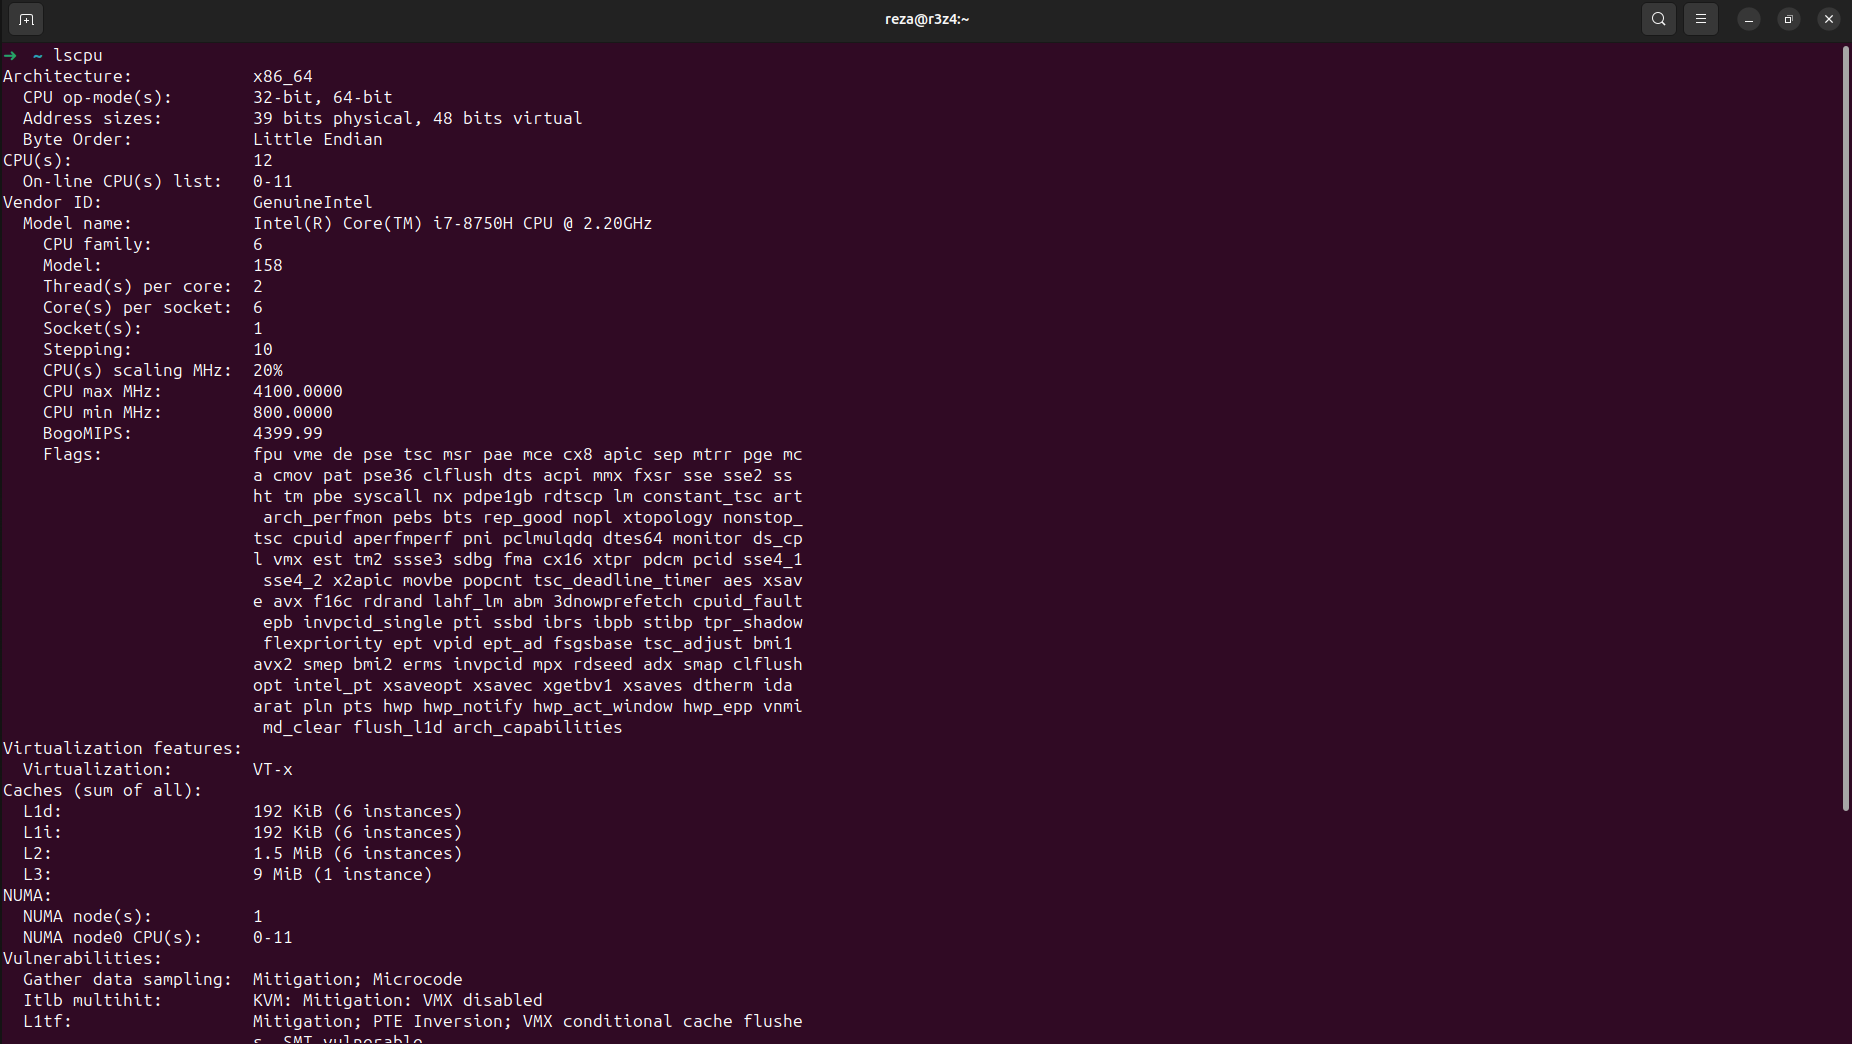
\includegraphics[width=\textwidth]{pics/img1.png}
	\end{center}
\end{qsolve}

دستور \texttt{top} یکی از ‫دستورات‬ ‫کاربردی‬ ‫در‬ ‫مدیریت‬ ‫پردازه‬ ‫هاست‪.‬‬ ‫این‬ ‫دستور‬ ‫اطلاعات‬ ‫مربوط‬ ‫به‬ \texttt{thread} های پردازنده، شماره پردازنده، ‫درصد‬ ‫استفاده‬ ‫از‬ ‫هر‬ ‫هسته‬ ‫پردازنده‬، ‫میزان‬ ‫استفاده‬ ‫هر‬ ‫پردازنده‬ ‫از‬ ‫کل‬ \texttt{cpu} و ... را به ما نشان می‌دهد. \\ \\ \\

‫این‬‫ دستور‬ ‫به‬ ‫صورت‬ ‫پیش‬ ‫فرض‬ ‫همه‬ ‫اطلاعات درمورد‬ ‫پردازه‬ ‫ها‬ ‫را‬ ‫به‬ ‫ما‬ ‫نمایش‬ ‫نمی‬ ‫دهد‬‫ اما‬ ‫می‌توانیم‬ ‫به‬ ‫صورت‬ ‫دستی‬‫ خودمان‬ ‫یک‬ ‫سری‬ ‫از‬ ‫اطلاعاتی‬ ‫که‬ ‫نیاز‬ ‫داریم‬ ‫را‬ ‫به‬ ‫ستون‬ ‫های‬ ‫اطلاعاتش‬ ‫اضافه‬ ‫و‬ ‫کم‬ ‫کنیم‪.‬‬ ‫برای‬ ‫اینکار‬ ‫پس‬ از‬‫ اجرای‬ \texttt{top} دکمه \texttt{f} را فشار دهید. ‫صفحه‬ ‫ای‬ ‫مشابه‬ ‫تصویر‬ ‫زیر‬ ‫برایتان‬ ‫نمایش‬ ‫داده‬ ‫میشود‬. با کلید‌های ‫بالا ‬‫و‬ ‫پایین‬ ‫کیبورد‬ ‫می‌توان‬ ‫در‬ ‫این‬ ‫گزینه‬‫ها‬ ‫جا‬ ‫به‬ ‫جا‬ ‫شد‬ ‫و‬ ‫با‬ ‫کلید‬ \texttt{space} می‌توان گزینه‌های مختلفی را انتخاب کرد.
\begin{qsolve}
	\begin{center}
		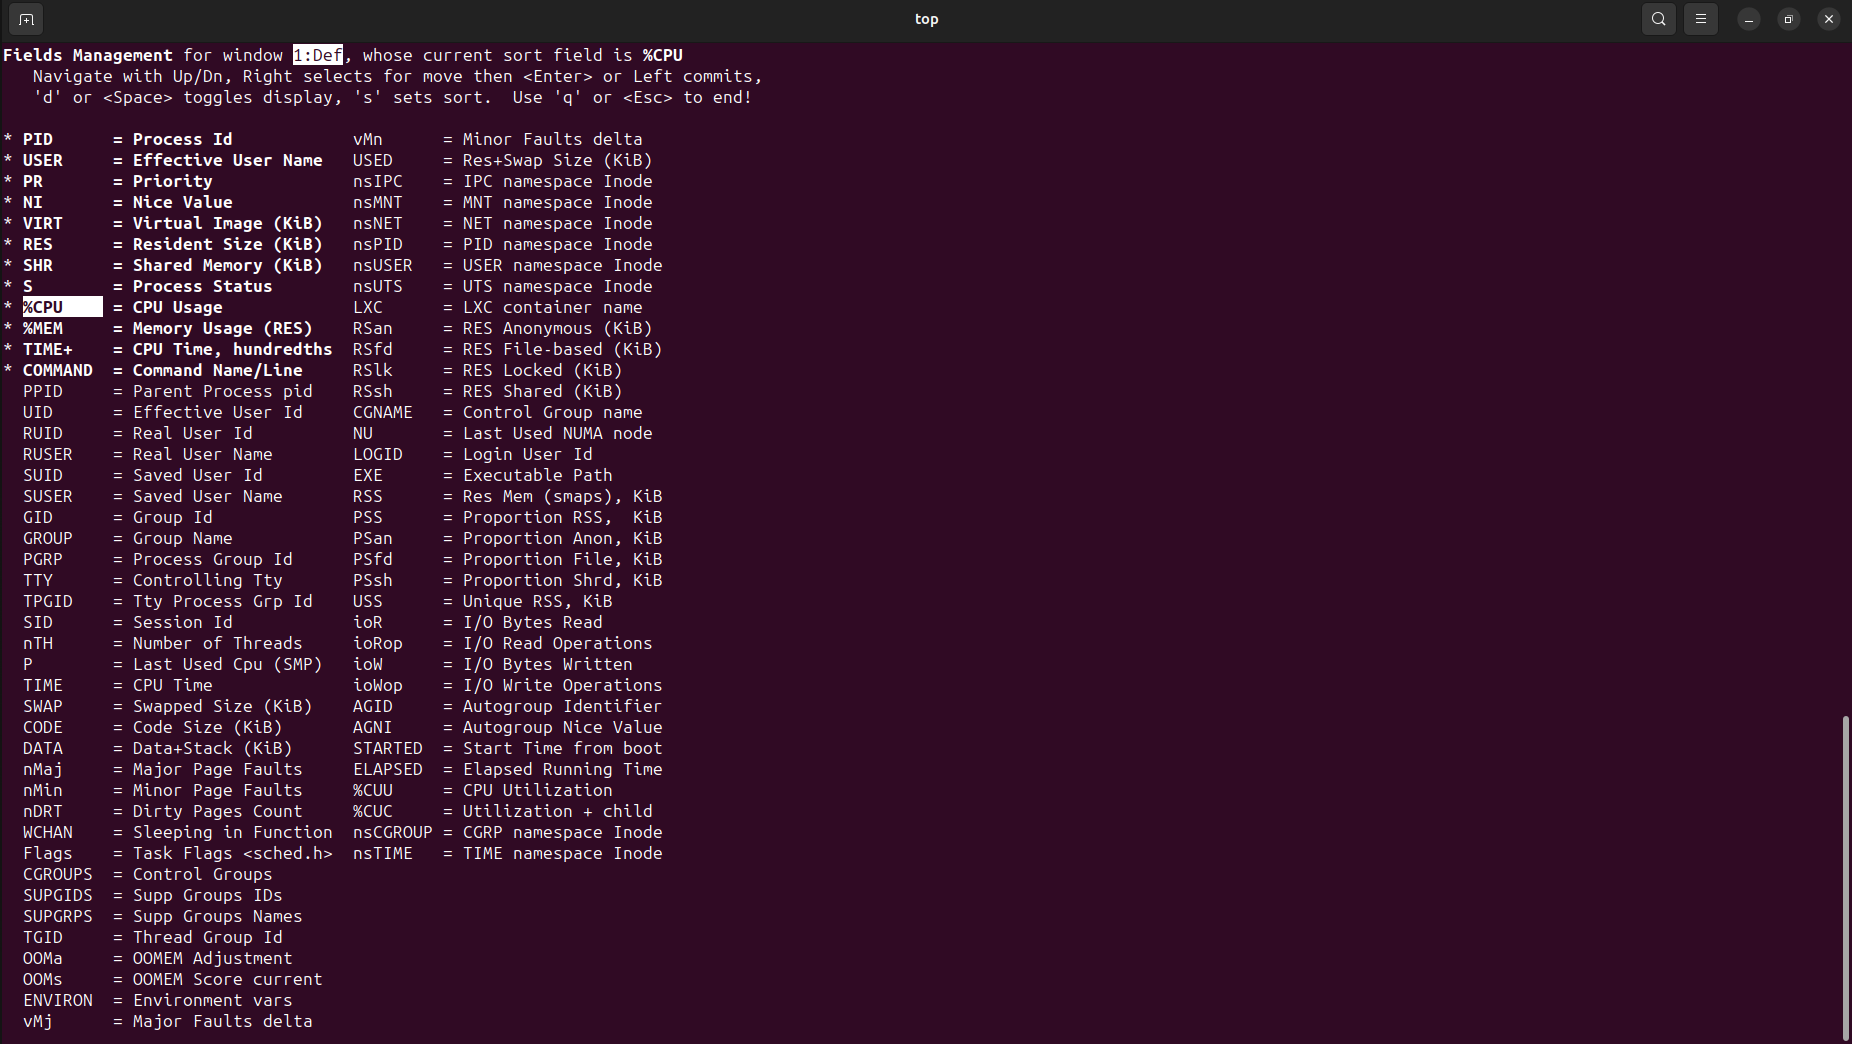
\includegraphics[width=\textwidth]{pics/img2.png}
	\end{center}
\end{qsolve}

\texttt{nTH} تعداد \texttt{thread} های یک پردازه و \texttt{p} ‫شماره‬ ‫آخرین‬ ‫هسته‬ ‫پردازنده‬ ‫ای‬ ‫که‬ ‫برای‬ ‫پردازه‬ ‫استفاده‬ ‫شده‬ ‫است‬ ‫را‬
‫نمایش ‬‫می‬ ‫دهد‪.‬‬‫ این‬ ‫دو‬ ‫گزینه‬ ‫را‬ ‫انتخاب‬ ‫کنید‬ ‫و‬ ‫خروجی‬ ‫آن‬ ‫را‬ ‫در‬ ‫گزارشتان‬ ‫بیاورید‪.‬‬

\begin{qsolve}
	\begin{center}
		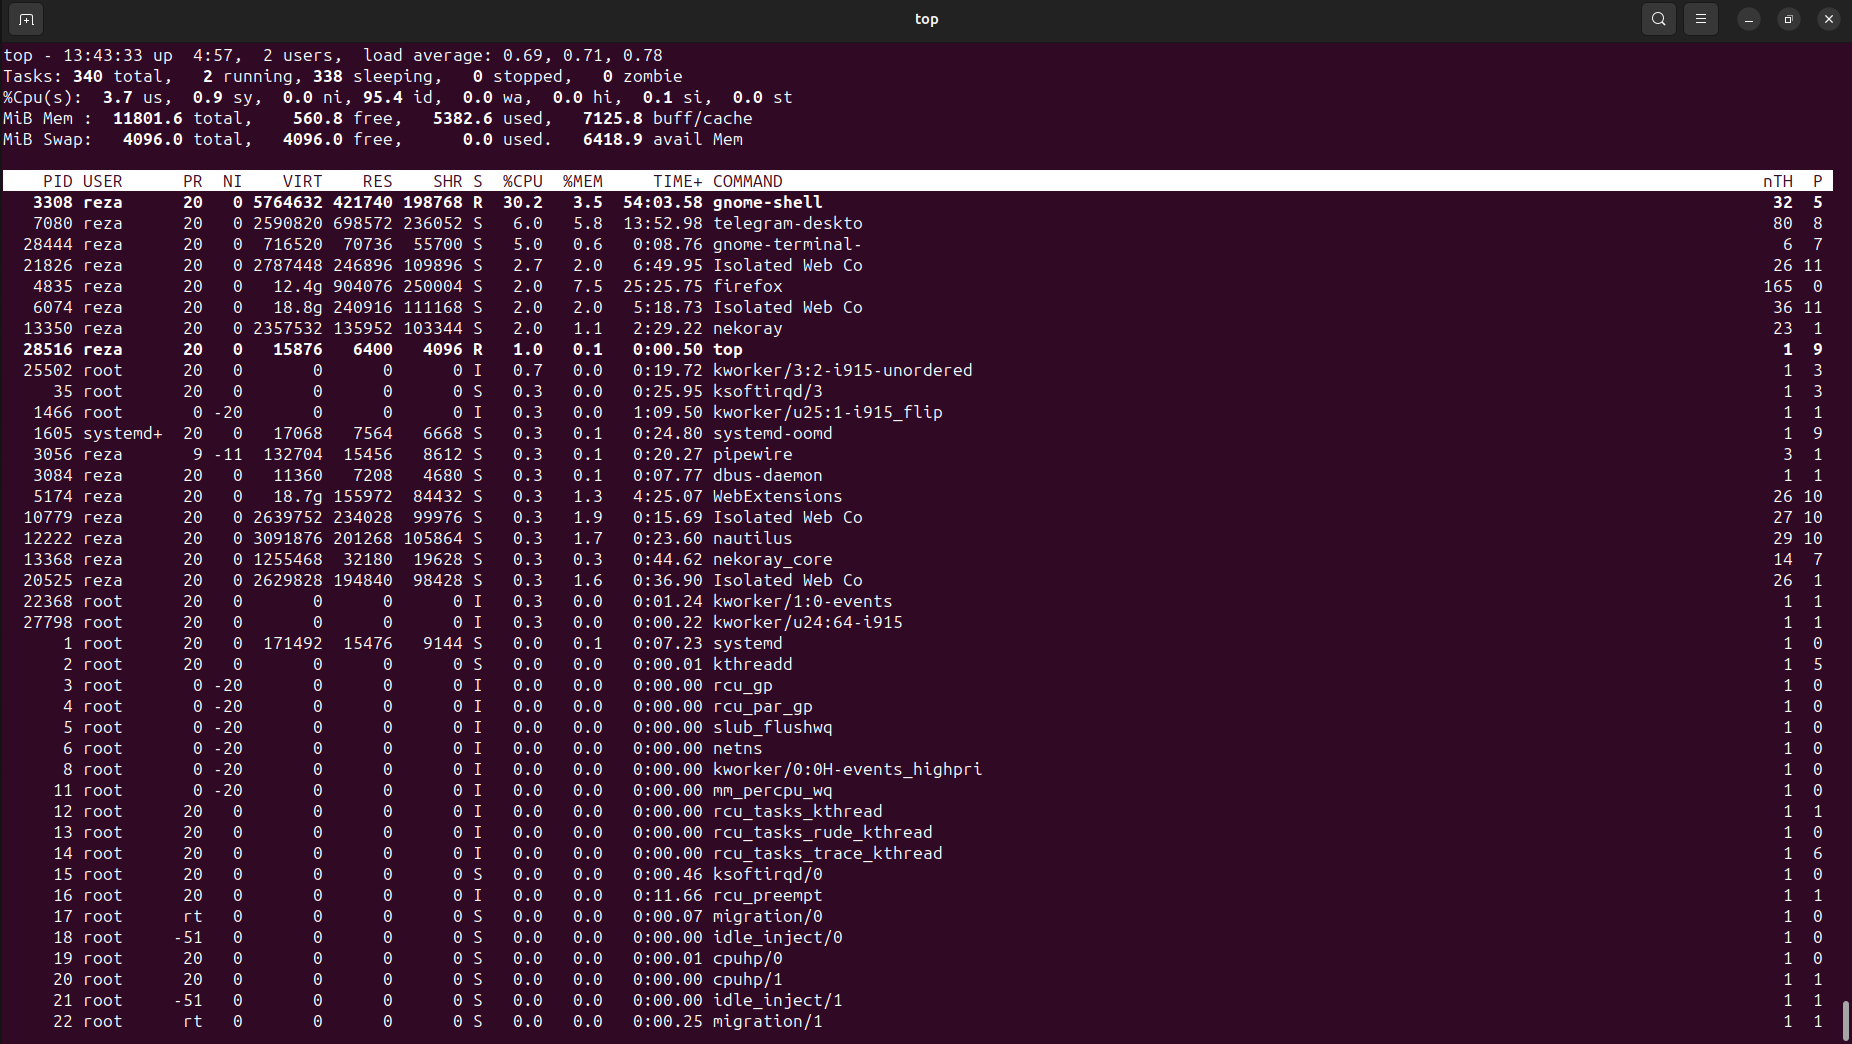
\includegraphics[width=\textwidth]{pics/img3.png}
	\end{center}
\end{qsolve}

همچنین با فشار دادن کلید ۱ در پردازه \textbf{top} ‫می‬ ‫توان‬ ‫میزان‬ ‫استفاده‬ ‫از‬ ‫هر‬ ‫کدام‬ ‫از‬ \texttt{core} های پردازه را مشاهده کرد.

\begin{qsolve}
	\begin{center}
		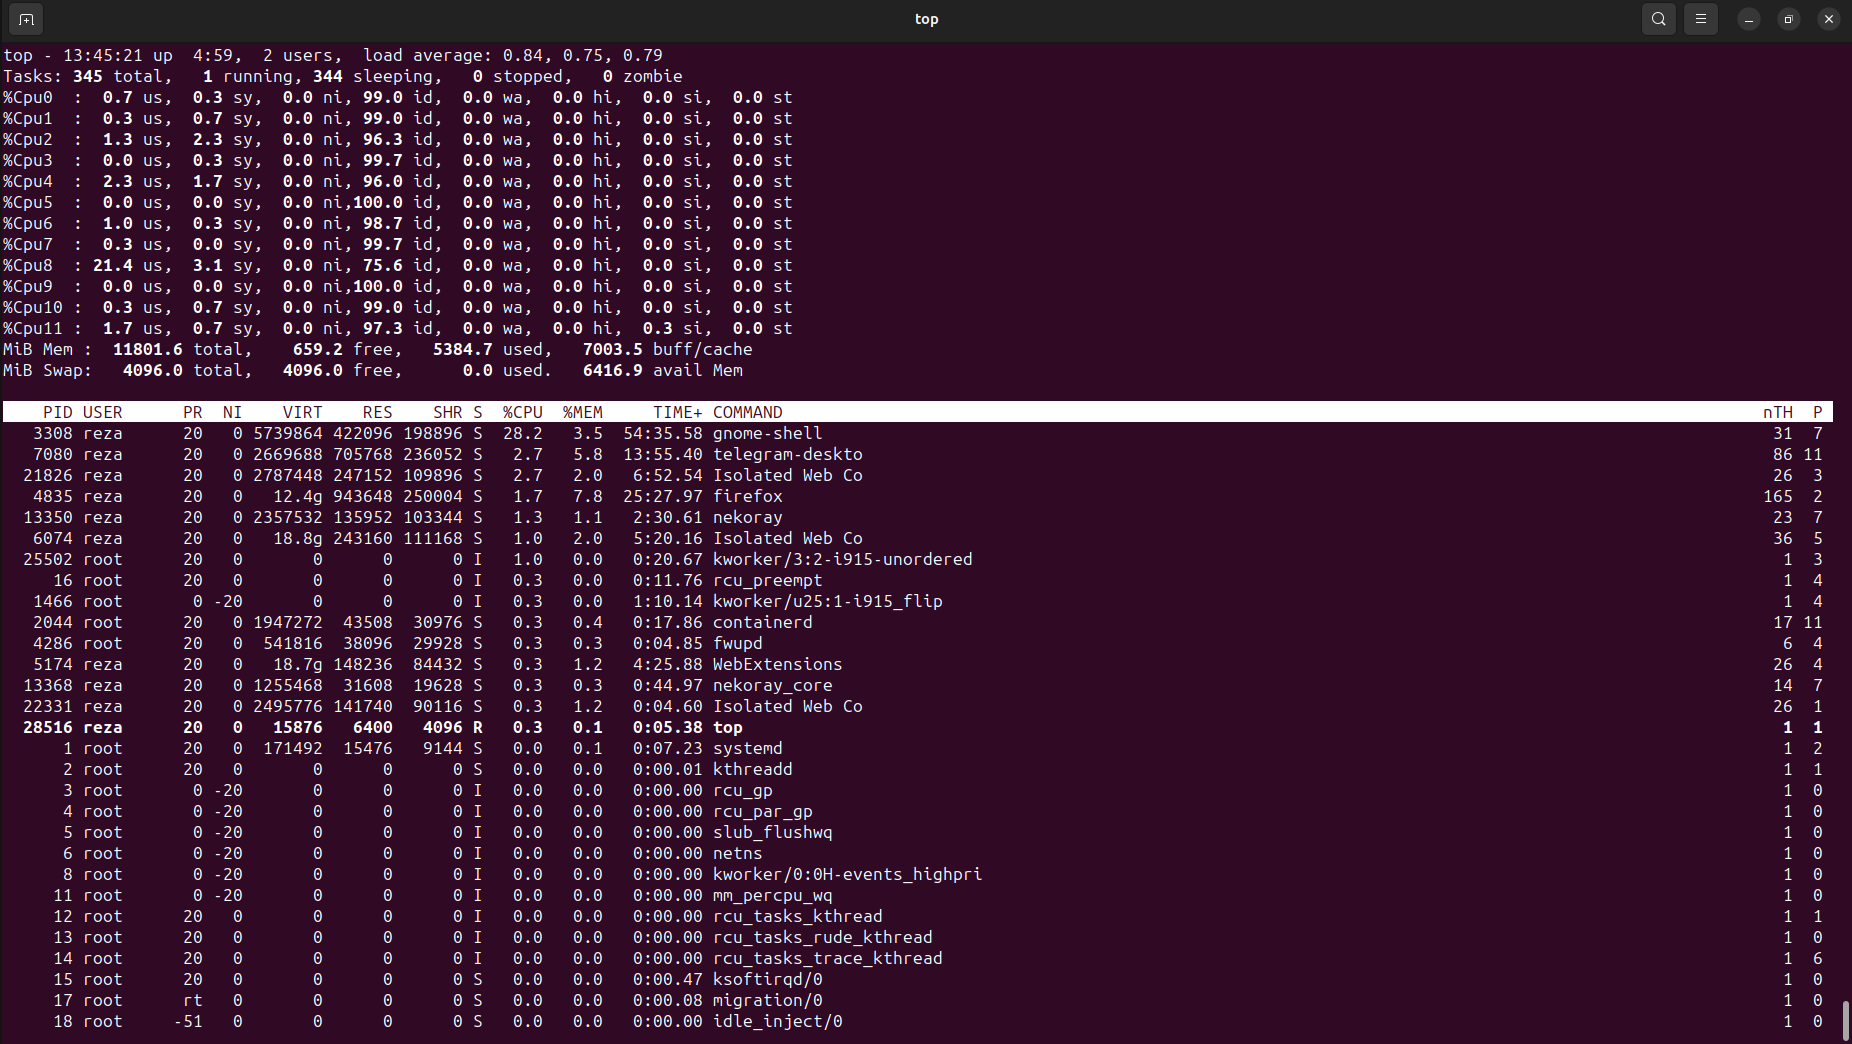
\includegraphics[width=\textwidth]{pics/img4.png}
	\end{center}
\end{qsolve}

‫گاهی ‬‫اوقات‬ ‫می‬ ‫خواهیم‬ ‫که‬ ‫یک‬ ‫پردازه‪،‬‬ ‫برای‬ ‫مدیریت‬ ‫بهتر‪،‬‬ ‫بر‬ ‫روی‬ ‫یک‬ \texttt{core} ‫از‬ ‫پردازنده‬ ‫اجرا‬ ‫شود‪.‬‬ ‫با‬ ‫دستور‬ \texttt{taskset} ‫میتوانیم‬ ‫مشخص‬ ‫کنیم‬ ‫که‬ ‫پردازه‬ ‫روی‬ ‫کدام‬ ‫یک‬ ‫از‬ ‫‪\texttt{core}‬‬ ‫های‬ ‫پردازنده‬ ‫اجرا‬ ‫شود‪.‬‬



